%% 
%% Copyright 2007-2025 Elsevier Ltd
%% 
%% This file is part of the 'Elsarticle Bundle'.
%% ---------------------------------------------
%% 
%% It may be distributed under the conditions of the LaTeX Project Public
%% License, either version 1.3 of this license or (at your option) any
%% later version.  The latest version of this license is in
%%    http://www.latex-project.org/lppl.txt
%% and version 1.3 or later is part of all distributions of LaTeX
%% version 1999/12/01 or later.
%% 
%% The list of all files belonging to the 'Elsarticle Bundle' is
%% given in the file `manifest.txt'.
%% 
%% Template article for Elsevier's document class `elsarticle'
%% with numbered style bibliographic references
%% SP 2008/03/01
%% $Id: elsarticle-template-num.tex 272 2025-01-09 17:36:26Z rishi $
%%
\documentclass[preprint,12pt]{elsarticle}

\usepackage{tabularx}
%% Use the option review to obtain double line spacing
%% \documentclass[authoryear,preprint,review,12pt]{elsarticle}

\usepackage{ragged2e}

%% Use the options 1p,twocolumn; 3p; 3p,twocolumn; 5p; or 5p,twocolumn
%% for a journal layout:
%% \documentclass[final,1p,times]{elsarticle}
%% \documentclass[final,1p,times,twocolumn]{elsarticle}
%% \documentclass[final,3p,times]{elsarticle}
%% \documentclass[final,3p,times,twocolumn]{elsarticle}
%% \documentclass[final,5p,times]{elsarticle}
%% \documentclass[final,5p,times,twocolumn]{elsarticle}

%% For including figures, graphicx.sty has been loaded in
%% elsarticle.cls. If you prefer to use the old commands
%% please give \usepackage{epsfig}

%% The amssymb package provides various useful mathematical symbols
\usepackage{amssymb}
%% The amsmath package provides various useful equation environments.
\usepackage{amsmath}
%% The amsthm package provides extended theorem environments
%% \usepackage{amsthm}


\journal{Nuclear Physics B}

\begin{document}

\begin{frontmatter}


\title{Integration of CBAM to Improve the Performance and Efficiency of MobileNetV3 for Fruit Plant Disease Classification Based on Leaf Symptoms}


\author[1]{Firmansyah Sundana} %% Author name
\author[1]{Fitri Utaminingrum} %% Author name
\author[1]{Budi Darma Setiawan} %% Author name

%% Author affiliation
\affiliation[1]{organization={Faculty of Computer Science, Brawijaya University},%Department and Organization
            addressline={}, 
            city={Malang},
            postcode={}, 
            state={East Java},
            country={Indonesia}}

%% Abstract
\begin{abstract}
Disease detection in fruit plants through leaf symptoms plays a crucial role in enhancing agricultural productivity. However, manual diagnosis often lacks efficiency and accuracy. This research proposes the integration of the Convolutional Block Attention Module (CBAM) into the MobileNetV3 architecture to improve the performance and efficiency of image-based plant disease classification. MobileNetV3 is chosen for its lightweight and efficient design, while CBAM enhances feature representation by applying attention mechanisms on both channel and spatial dimensions. The study utilizes the PlantVillage dataset, which includes 29 classes of fruit plant leaf images. Evaluations are conducted on performance metrics (accuracy, precision, recall, and F1-score), complexity metrics (Floating Point Operations, number of parameters, memory size), and efficiency metrics (training time, inference time, latency, and throughput). Results show that integrating CBAM consistently improves classification accuracy and inference efficiency compared to standard MobileNetV3, with minimal additional computational cost. This study contributes to the development of lightweight, accurate, and deployable plant disease classification systems for mobile and edge devices.
\end{abstract}

%%Graphical abstract
\begin{graphicalabstract}
%\includegraphics{grabs}
\end{graphicalabstract}

%%Research highlights
\begin{highlights}
\item CBAM enhances MobileNetV3 accuracy for plant diseases classification.
\item Integration of CBAM reduces MobileNetV3 model complexity.
\item CBAM integration significantly improves MobileNetV3 inference efficiency.
\item Faster training times achieved with MobileNetV3 Small + CBAM r32.
\end{highlights}

%% Keywords
\begin{keyword}
%% keywords here, in the form: keyword \sep keyword
plant disease classification, computer vision, deep learning, MobileNetV3, CBAM


\end{keyword}

\end{frontmatter}


%% Use \section commands to start a section
\section{Introduction}
\label{sec1}
%% Labels are used to cross-reference an item using \ref command.

Global food security and nutrition heavily rely on fruit plant cultivation, yet plant diseases frequently cause significant economic losses for farmers. Traditional disease identification methods, relying on manual diagnosis by agronomists, are often time-consuming, expensive, and prone to inaccuracies due to subjective factors and limited expert availability \cite{Sajitha2024, Wang2024}. This scarcity of agricultural experts, particularly in remote areas, often leads to delayed disease management and substantial crop losses.

To mitigate these challenges, precision agriculture systems are increasingly being adopted \cite{Laveglia2024}. These systems utilize advanced technologies like sensors, cameras, and drones to gather real-time farmland data, aiding in tasks such as irrigation scheduling, fertilization, microclimate monitoring, and crucial plant health evaluation \cite{Balafas2023}. Specifically, integrating digital cameras within these systems offers immense potential for automated and efficient detection and classification of fruit plant diseases.

Recent advancements in computer vision and deep learning have provided innovative solutions for automated plant disease classification, with studies demonstrating high accuracy, often exceeding 90\% \cite{Lu2025,Sajitha2024, Pandian2022, Syed-Ab-Rahman2022}. Convolutional Neural Networks (CNNs), in particular, have proven highly effective in analyzing plant leaf images for disease symptoms \cite{Vishnoi2023}.

Despite promising theoretical performance, a significant gap exists between deep learning's capabilities and practical, real-world implementation. A primary challenge is the high computational resource requirement of these models, leading to suboptimal performance on resource-constrained hardware like mobile or edge devices \cite{Liu2023}. Evaluating computational efficiency involves metrics such as Floating Point Operations (FLOPs), number of parameters, model memory size, and temporal aspects like training/testing time, latency, and throughput \cite{Menghani2023,Qi2022}.

Current research often prioritizes either accuracy or computational efficiency, with limited comprehensive exploration into integrating efficient attention mechanisms within lightweight architectures specifically for fruit plant disease classification. This research gap hinders practical field implementation, especially in regions with limited technological infrastructure.

This study proposes an innovative solution by integrating the Convolutional Block Attention Module (CBAM) into the MobileNetV3 architecture to develop a more effective and efficient model for fruit plant disease classification. MobileNetV3 is specifically designed for efficiency in terms of parameters and computational power, making it suitable for resource-constrained devices due to its separable convolution techniques and inverted residual-based architecture \cite{Howard2019, Maharani2025}. CBAM enhances the model's ability to extract more relevant features by sequentially applying attention mechanisms to both spatial and channel dimensions, unlike other attention mechanisms that may focus solely on one dimension \cite{MuhammadAlqadri2024, Woo2018, Zhang2022}. This approach allows CBAM to reduce additional parameters and computational burden while maintaining focus on important features \cite{Zhang2021, Zhang2022}.

Previous research has demonstrated the individual potential of these two approaches. MobileNetV3 has shown competitive accuracy and efficiency for corn plant disease classification \cite{Syaharani2023}, while CBAM has effectively extracted relevant features in complex environments like human face pose classification \cite{Chen2022}. By combining the strengths of MobileNetV3 and CBAM, this research aims to develop a robust model for fruit plant disease classification. We utilize the PlantVillage dataset, a widely accepted benchmark for plant disease classification, focusing on leaf images from various fruit plants, including apple, blueberry, cherry, grape, orange, peach, raspberry, strawberry, squash, and tomato. This research is expected to significantly contribute to the development of accurate, efficient, and reliable deep learning-based plant disease classification technology, offering a practical solution for field implementation with limited computational resources.

\section{Methods and Implementation}

This section details the research methodology, encompassing the experimental design, data collection and preprocessing, model architecture, experimental setup, and evaluation metrics employed in this study. The whole process of this research is shown in Figure \ref{fig1: research-workflow}.

\begin{figure}[t]
\centering
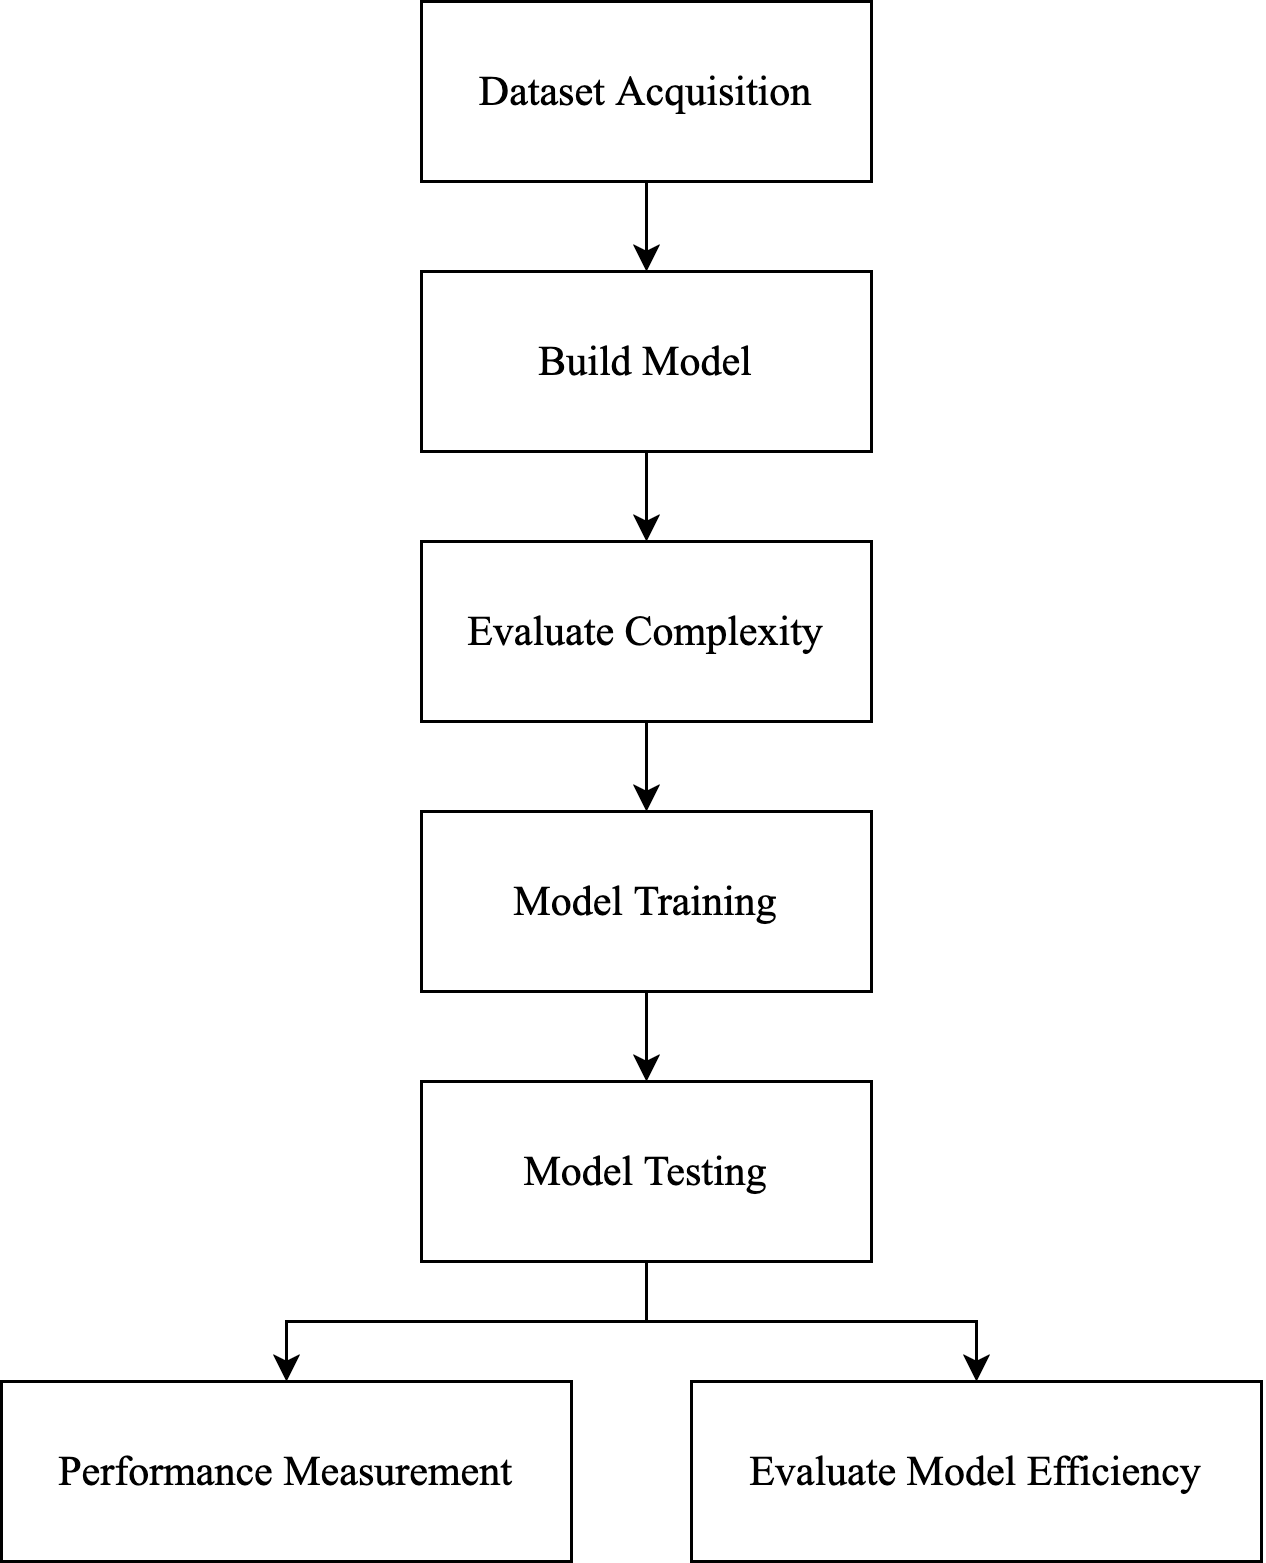
\includegraphics[width=0.5\textwidth]{research-flowchart-paper.png}
\caption{Research workflow}\label{fig1: research-workflow}
\end{figure}

\subsection{Data Collection and Preprocessing}

\subsubsection{Dataset}

The PlantVillage dataset was utilized for this research, a publicly available and widely recognized dataset for plant disease classification. This dataset comprises images of plant leaves exhibiting disease symptoms and healthy conditions. For this study, 29 specific classes of fruit plant diseases and healthy leaves were selected from the PlantVillage dataset. These classes include diseases and healthy samples from apple, blueberry, cherry, grape, orange, peach, raspberry, strawberry, squash, and tomato plants. The dataset totals 46,565 images.

The dataset was partitioned into three sets: 70\% for training, 15\% for validation, and 15\% for testing. Each image was resized to 224×224 pixels and converted into a tensor format suitable for deep learning models.

\begin{figure}[t]
    \centering
    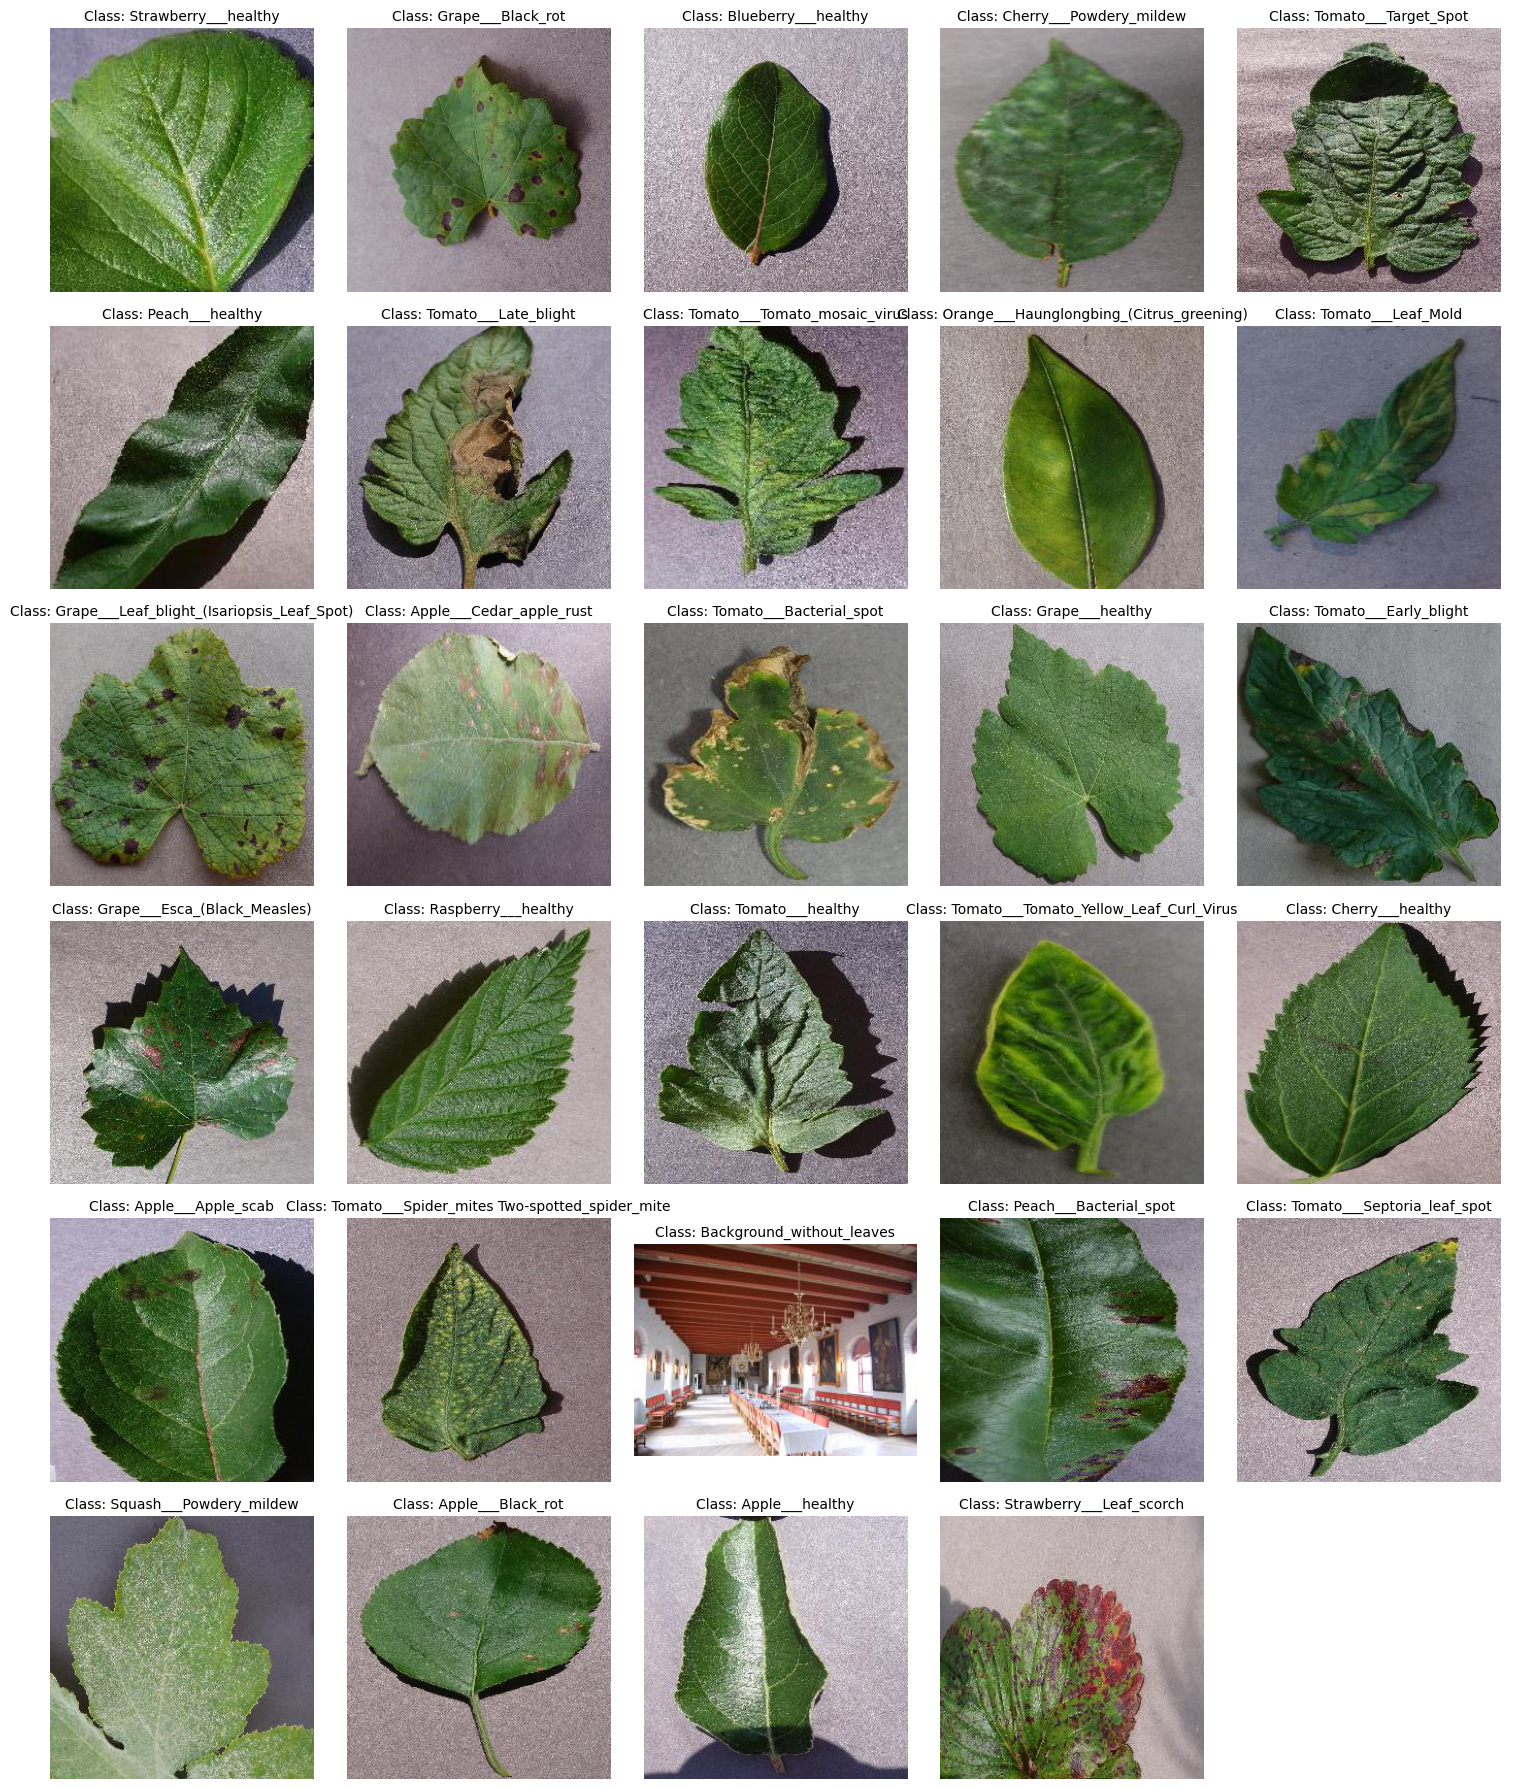
\includegraphics[width=\textwidth]{dataset.png}
    \caption{Image sample for each class in PlantVillage.}
    \label{fig:dataset}
\end{figure}

\subsection{Model Architecture}

This study proposes an integration of the Convolutional Block Attention Module (CBAM) into the MobileNetV3 architecture. Two variants of MobileNetV3, Large and Small, were used as baseline models for comparison as shown in Figure \ref{fig:mobilenet3-arch}.

\subsubsection{MobileNetV3 Baseline}

The baseline MobileNetV3 architecture (both Large and Small variants) utilizes an initial 3×3 convolutional layer followed by Batch Normalization (BN) and h-Swish activation. The core of MobileNetV3 comprises a sequence of "inverted residual blocks" which include a 1×1 expansion convolution, a depthwise separable convolution, a Squeeze-and-Excitation (SE) module, and a 1×1 projection layer. A final 1×1 convolutional layer processes the features before the classification head. Skip connections are employed when input and output dimensions are compatible.

\subsubsection{MobileNetV3 with CBAM Integration}

In the proposed model, the Squeeze-and-Excitation (SE) module within the inverted residual blocks of MobileNetV3 (both Large and Small variants) is replaced with the Convolutional Block Attention Module (CBAM). CBAM sequentially applies channel attention and spatial attention to refine feature maps. Channel attention pools spatial information to generate channel-wise attention weights, while spatial attention highlights significant areas within the spatial dimensions of the feature map. The integration was tested with two reduction ratios for CBAM: 16 and 32, to evaluate their impact on model performance and efficiency.

\begin{figure}[t]
    \centering
    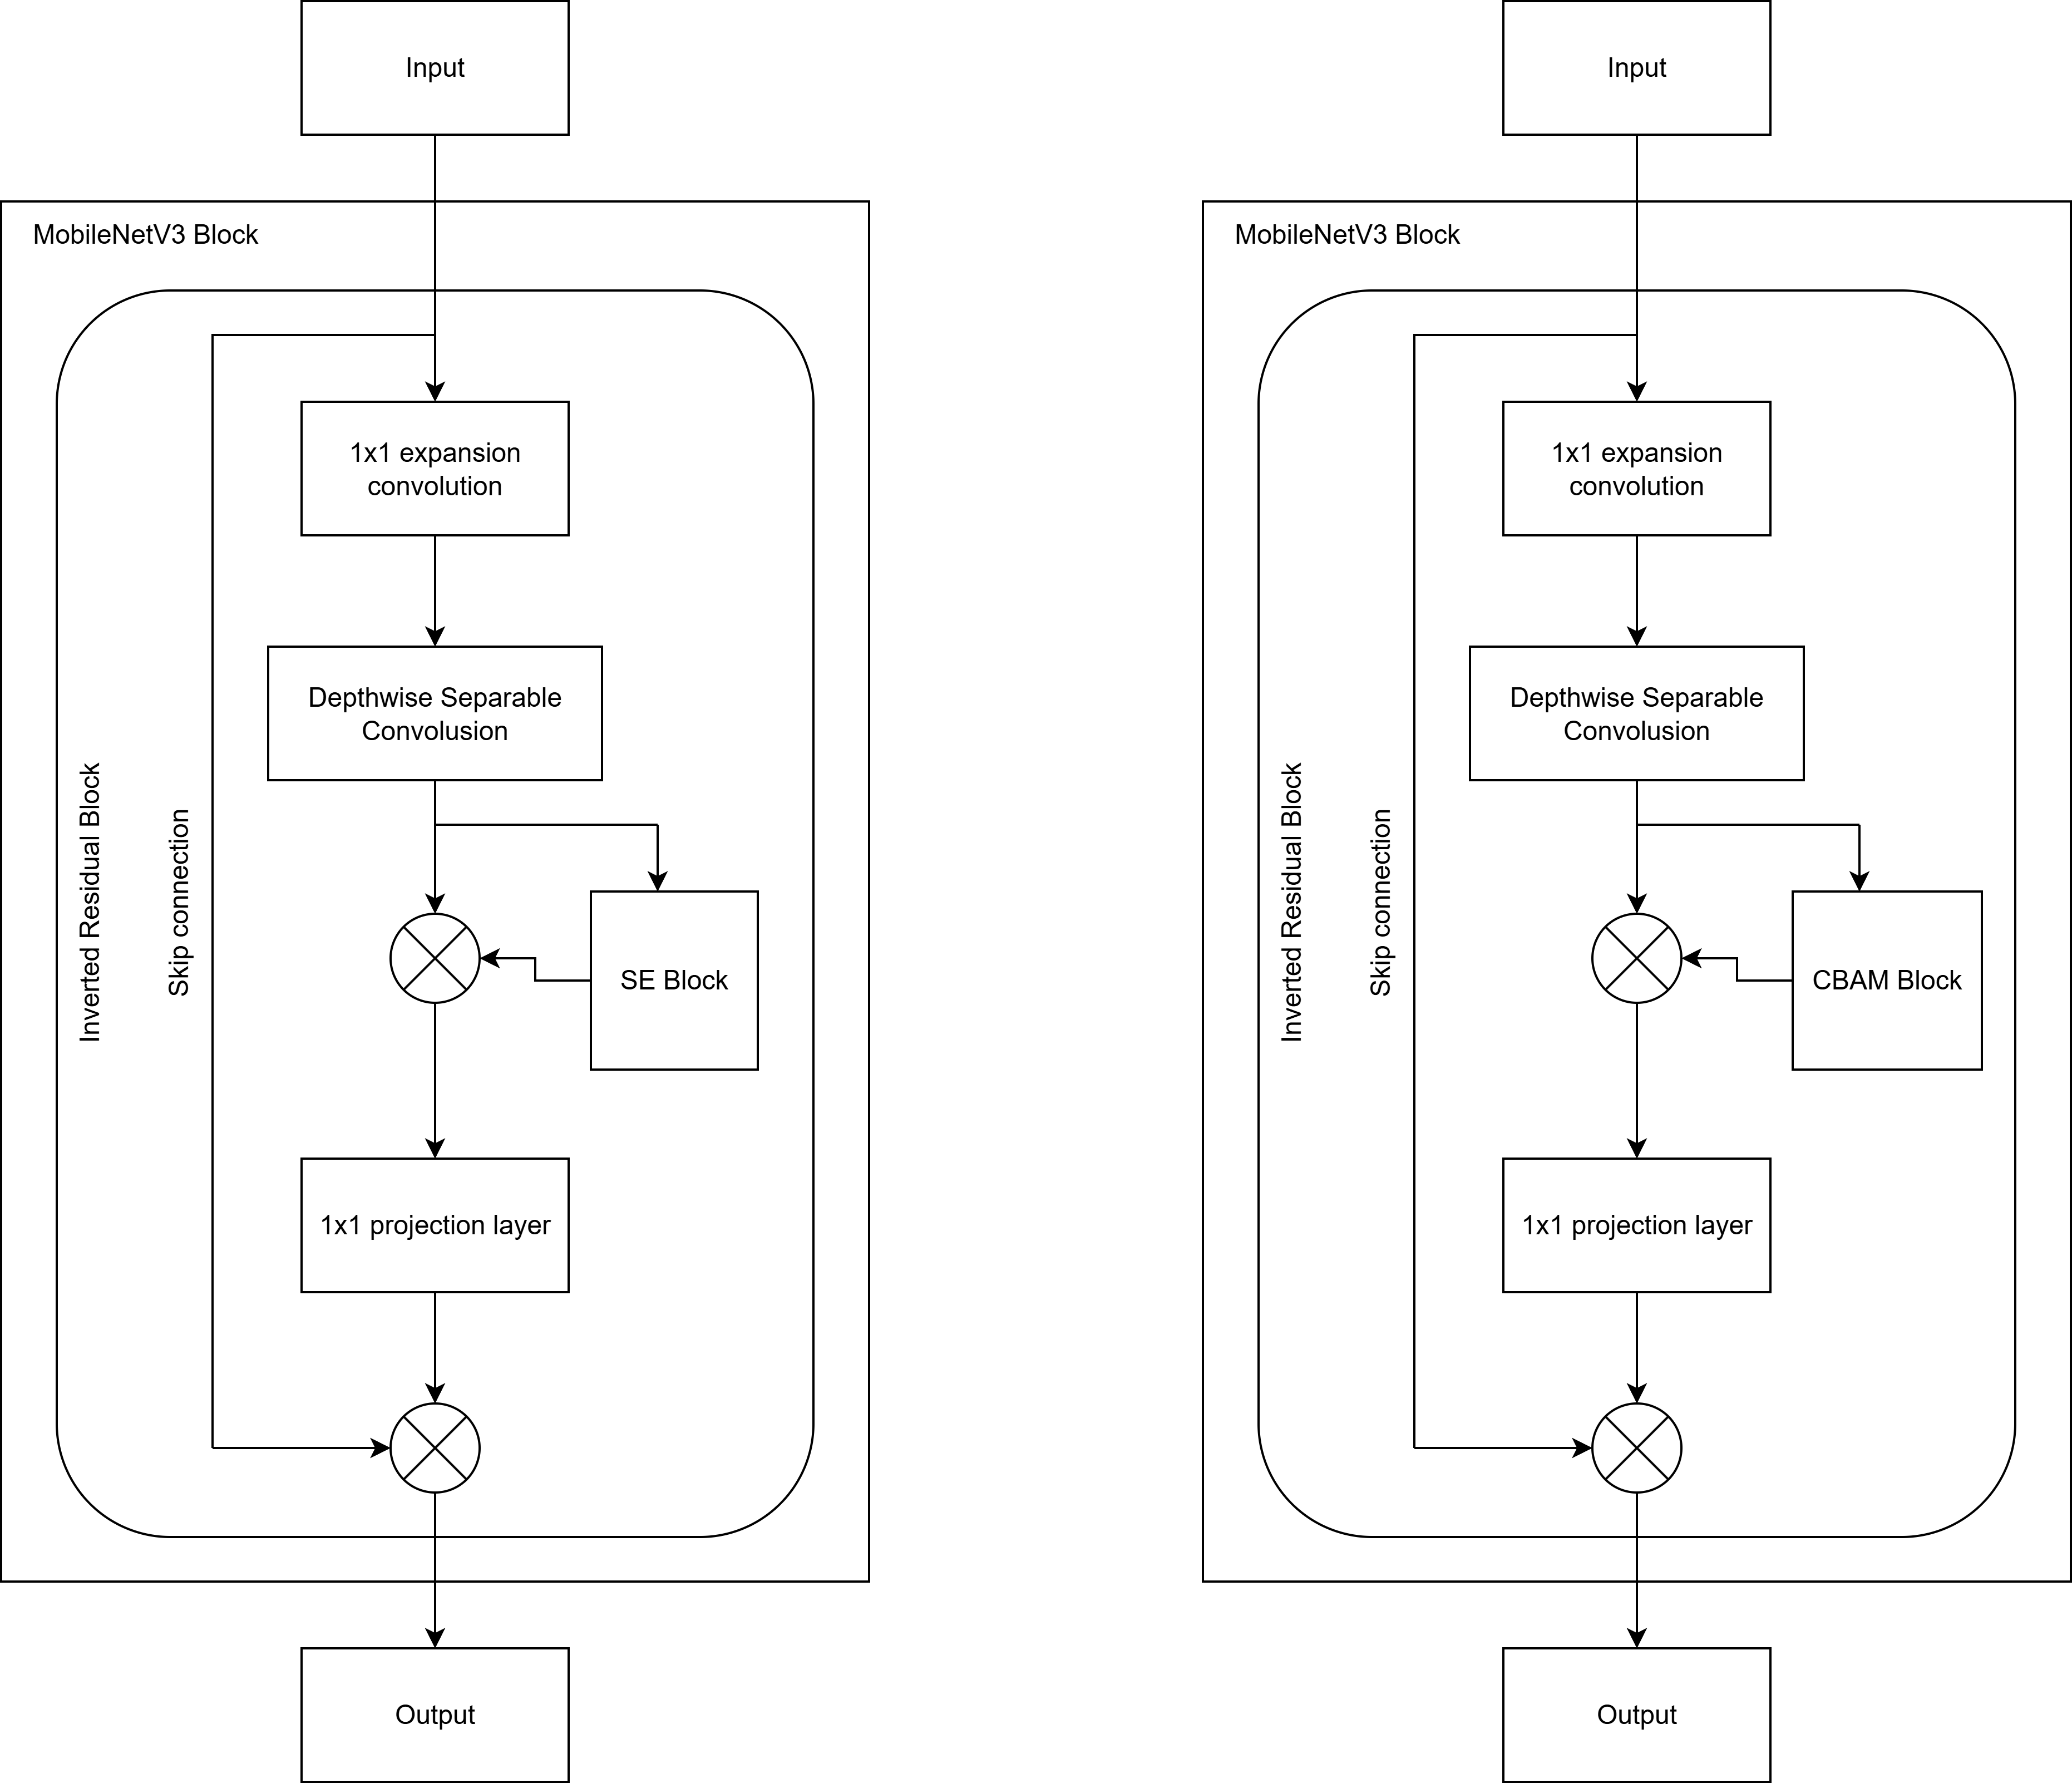
\includegraphics[width=\linewidth]{MobileNetV3+CBAM.png}
    \caption{Left: MobileNetV3 Block baseline architecture using SE Block. Right: MobileNetV3 Block using CBAM as its attention module.}
    \label{fig:mobilenet3-arch}
\end{figure}

\subsection{Hyperparameter Initialization}

The following hyperparameters were configured prior to the training process:

\begin{enumerate}
    \item Learning Rate: 0.001
    \item Batch Size: 64
    \item Optimizer: Adam
    \item Loss Function: Cross Entropy Loss
\end{enumerate}

The Adam optimizer was chosen for its rapid convergence and minimal tuning requirements compared to Stochastic Gradient Descent (SGD). Cross Entropy Loss was selected as it is highly suitable for multi-class classification problems, directly measuring the alignment between predicted probability distributions and true labels.

\subsection{Training and Testing Algorithms}

\subsubsection{Training Algorithm}

Model training involved an iterative process where models learned from the training data, adjusted parameters through backpropagation using the Adam optimizer, and evaluated performance on the validation set. An Early Stopping algorithm was implemented to automatically halt the training process if a predefined stopping criterion was met. This criterion was based on the absence of significant improvement in validation loss over a set number of epochs, preventing overfitting. During each epoch, a forward pass was performed on the training data to compute the loss, followed by a backward pass to update weights. Subsequently, a forward pass on the validation data was conducted to monitor accuracy and loss. The model weights corresponding to the best validation performance were saved.

\subsubsection{Testing Algorithm}

Following training, the model with the best-performing weights (identified via Early Stopping) was evaluated on the unseen test dataset. During the testing phase, only a forward pass was performed, as weight updates (backpropagation) were no longer necessary. The predictions generated were then used to calculate various performance and efficiency metrics.

\subsection{Evaluation Metrics}

Model performance was comprehensively evaluated using a combination of classification metrics, complexity metrics, and efficiency metrics.

\subsubsection{Performance Metrics}

For multi-class classification, the following standard metrics were computed for each class and then averaged. Accuracy quantifies the proportion of correctly predicted instances relative to the total number of instances, as defined in Equation \eqref{eq:accuracy}. Precision indicates the proportion of true positive predictions among all instances predicted as positive, as shown in Equation \eqref{eq:precision}. Recall measures the proportion of true positive predictions among all actual positive instances, described by Equation \eqref{eq:recall}. The F1-score, calculated as the harmonic mean of precision and recall, offers a balanced measure of the model's performance, as given in Equation \eqref{eq:f1score}, where TP is True Positive, TN is True Negative, FP is False Positive, and FN is False Negative.

\begin{equation}
    Accuracy= \frac{TP+TN}{TP+TN+FP+FN}
    \label{eq:accuracy}
\end{equation}

\begin{equation}
    Precision_i=\frac{TP}{TP+FP}
    \label{eq:precision}
\end{equation}

\begin{equation}
    Recall=\frac{TP}{TP+FN}
    \label{eq:recall}
\end{equation}

\begin{equation}
    F1score=2\times\frac{Precision \times Recall}{Precision + Recall}
    \label{eq:f1score}
\end{equation}


\subsubsection{Complexity Metrics}

Model complexity was assessed based on Floating Point Operations (FLOPs). It quantifies the total number of floating-point arithmetic operations (additions, subtractions, multiplications, divisions) performed by the model during inference. It was also calculated for convolutional layers, fully connected layers, and batch normalization layers. Convolutional Layer FLOPs as calculated using Equation \ref{eq:convolution-flops}. Fully Connected Layer FLOPs, $2 \times \hat{X} \times \hat{Y}$. Batch Normalization FLOPs, $4 \times H \times W \times C$. Number of Parameters is a total count of internal variables learned by the model from the dataset during training. Calculated for fully connected layers, convolutional layers, and batch normalization layers. Fully Connected Layer Parameters, $(M \times N)+N$. Convolutional Layer Parameters, $(C_{in} \times K_H \times K_W \times C_{out})+B$. Batch Normalization Parameters, $2 \times C$. Model Memory Size (MB) is the memory footprint required to store the model's parameters and activations. Where, $C_{in}$ is channel input, $C_{out}$ is channel output, $H_{out}$ and $W_{out}$ are 2D output dimension, $K_H$ and $K_W$ are 2D kernel dimension. $\hat{X}$ and $\hat{Y}$ are both represent the number of input and output features (or dimensions). $M$ represents the number of neurons in the input layer to to the fully connected layer, $N$ represents the numbers of neurons or features in the current fully connected layer. This was calculated by summing the total number of parameters and multiplying by 4 bytes (assuming 32-bit precision), then converting to megabytes.

\begin{equation}
    \text{Convolution FLOPs} = 2 \times C_{in} \times H_{out} \times W_{out} \times K_H \times K_W \times C_{out}
    \label{eq:convolution-flops}
\end{equation}


\subsubsection{Efficiency Metrics}

Model efficiency was evaluated based on four key temporal metrics. Training Time (minutes) quantifies the total duration required for the model to converge during the learning process. Testing Time (ms) measures the time for the trained model to perform inference on new data. Latency (s/batch) represents the time delay from input reception to output generation, with measurements taken per batch (batch size of 64). Lastly, Throughput (samples/second) indicates the number of data samples the model can process per unit of time, reflecting its capacity for handling large-scale or real-time applications.

\section{Results and Discussion}

This section provides an overview of the experimental results from the evaluation of six deep learning models. The models assessed are MobileNetV3 (Large and Small variants), both with and without the integration of the Convolutional Block Attention Module (CBAM). The CBAM was evaluated at two different reduction ratios, 16 and 32. The analysis directly addresses the key research questions by examining three critical performance categories: performance, complexity, and efficiency metrics.

\subsection{Training and Validation Performance}

\begin{figure}[t]
    \centering
    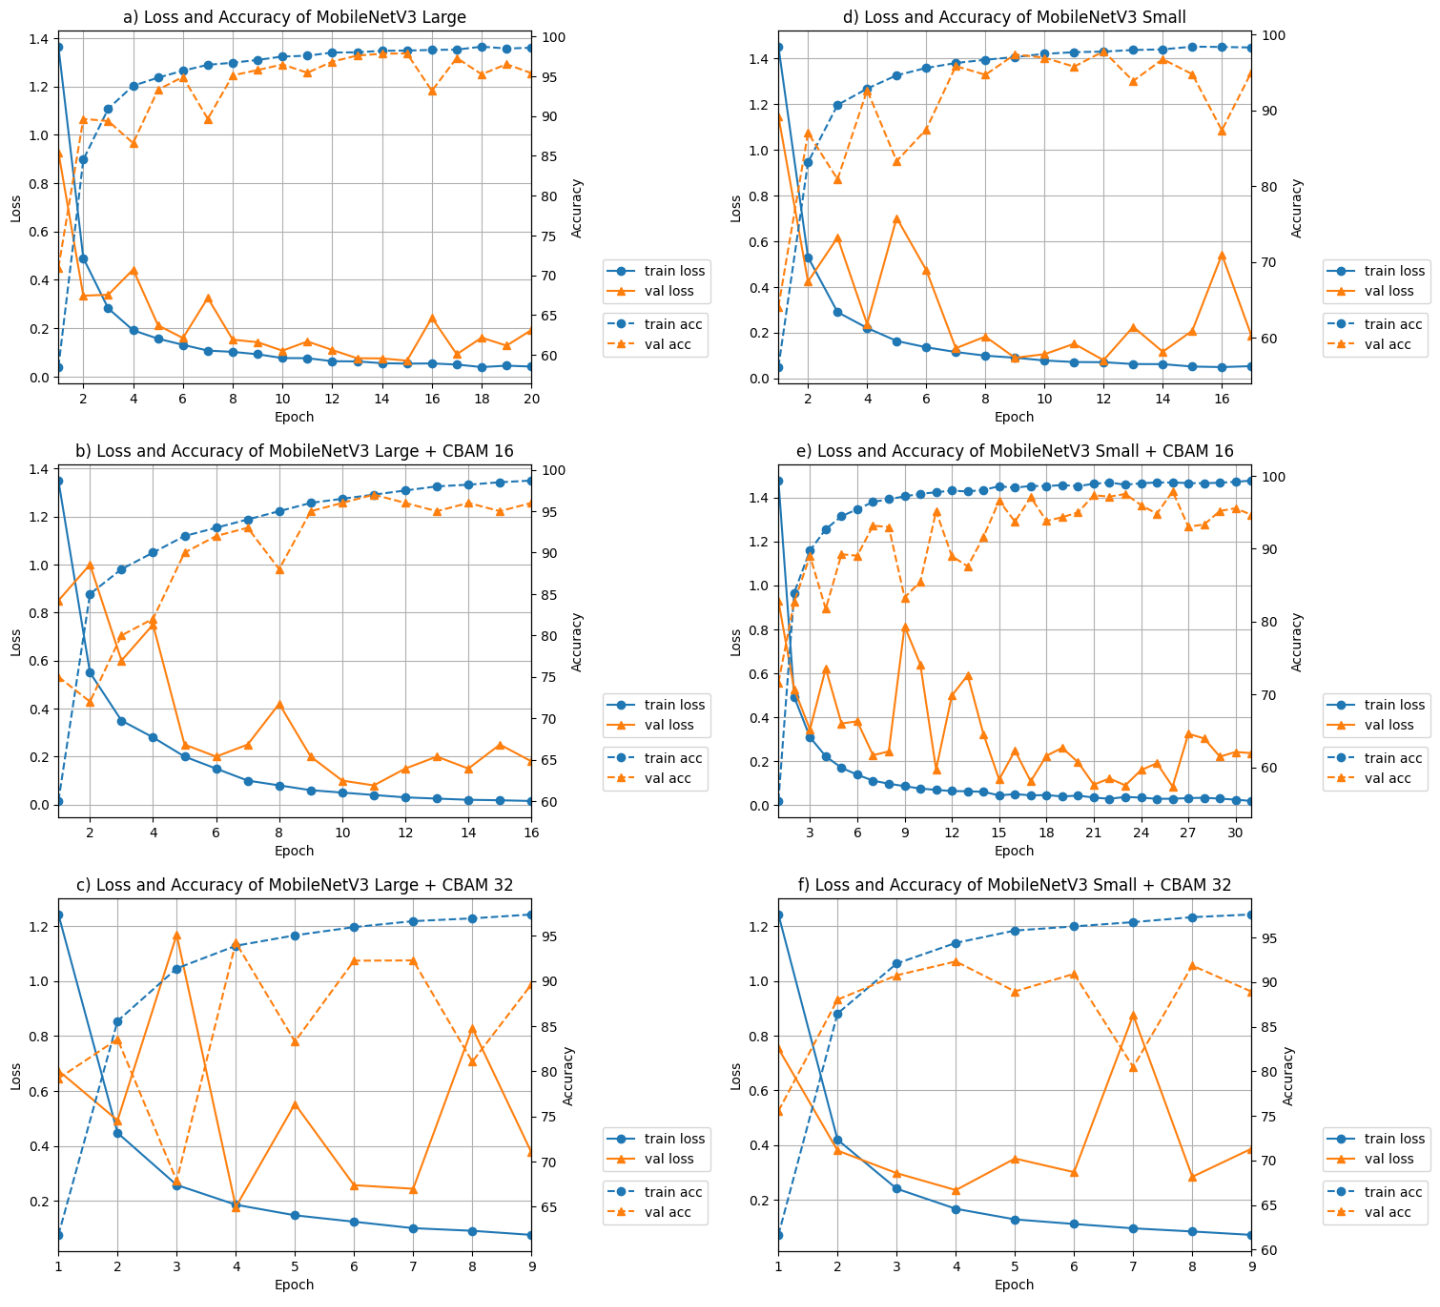
\includegraphics[width=0.95\linewidth]{training_log_graph.png}
    \caption{Training and Validation Performance of MobileNetV3 and
MobileNetV3+CBAM Variants.}
    \label{fig:train-log}
\end{figure}

The training process for each model variant began from scratch, with an early stopping algorithm determining the optimal epoch for model saving. For MobileNetV3 Large training concluded at epoch 20, though optimal generalization, marked by minimal validation loss and peak validation accuracy mirroring training accuracy, was observed around epoch 15. Fluctuations after epoch 15 hinted at early overfitting, as shown in Figure \ref{fig:train-log}a. The MobileNetV3 Large + CBAM r16 variant trained for 16 epochs, described in Figure \ref{fig:train-log}b. While training metrics consistently improved, validation loss and accuracy showed notable fluctuations at epoch 2 to 5. Small difference happened at epoch 11 between train and validation accuracy. In contrast, MobileNetV3 Large + CBAM r32 completed training in just 9 epochs, as shown in Figure \ref{fig:train-log}c. Despite a steady decrease in training loss, validation loss and accuracy exhibited sharp fluctuations, with peaks in loss at epochs 3 and 8, suggesting that a higher reduction ratio (32) might introduce instability in generalization and potential overfitting.

The MobileNetV3 Small variant trained for 17 epochs, demonstrating stable and convincing performance, as shown in Figure \ref{fig:train-log}d. Both training and validation accuracies consistently increased, with validation stabilizing above 90\% with only minor fluctuations. Correspondingly, training and validation losses showed positive downward trends, indicating a good balance between complexity and performance for this lightweight architecture. For MobileNetV3 Small + CBAM r16, training extended for 30 epochs, as shown in Figure \ref{fig:train-log}e. Training accuracy approached 100\%, and validation accuracy largely remained between 85\% and 99\%. However, significant fluctuations in validation loss and accuracy were observed, particularly in the early to mid-training stages (epochs 5-15), suggesting that while CBAM (r16) enhanced feature learning, further hyperparameter tuning or regularization might be needed for improved stability. Finally, training for the MobileNetV3 Small + CBAM r32 variant concluded at 9 epochs, as shown in Figure \ref{fig:train-log}f. Although training loss decreased smoothly, validation loss showed substantial fluctuations, peaking at epoch 7, and validation accuracy also fluctuated, indicating potential overfitting after initial epochs where improved training performance did not consistently translate to validation.

\subsection{Impact of CBAM on Performance Metrics}

The performance of all six models was evaluated using accuracy, precision, recall, and F1-score, along with confusion matrices.

The confusion matrices revealed consistent performance patterns across the MobileNetV3 Large variants (baseline, +CBAM r16, +CBAM r32), with dominant diagonal lines indicating accurate predictions.
 Notably, two classes, 'Haunglongbing (citrus greening)' on orange and 'Yellow leaf curl virus' on tomato, consistently showed darker intensities due to larger dataset sizes, implying higher prediction confidence for these classes. Similar diagonal patterns were observed for MobileNetV3 Small variants. However, MobileNetV3 Small + CBAM r32 showed relatively more misclassifications, particularly confusing healthy grape images with healthy strawberry plants, and misclassifying tomato target spot disease with healthy tomatoes 25 times.

\begin{table}[t]
\centering
    \begin{tabularx}{\textwidth}{ |l|X|X|X|X| }
     \hline
     \textbf{Model} & \textbf{Accuracy} & \textbf{Precision} & \textbf{Recall} & \textbf{F1-score} \\
     \hline
     Base Large & 0.98 & 0.98 & 0.98 & 0.9810 \\
     Base Large +CBAM r16 & 0.98 & 0.98 & 0.98 & 0.9806 \\
     Base Large +CBAM r32 & 0.96 & 0.96 & 0.96 & 0.9554 \\
     \hline
     Base Small & 0.98 & 0.98 & 0.98 & 0.9754 \\
     Base Small +CBAM r16 & 0.99 & 0.99 & 0.99 & 0.9873 \\
     Base Small +CBAM r32 & 0.93 & 0.94 & 0.93 & 0.9346 \\
     \hline
    \end{tabularx}
    \caption{Performance Metrics of MobileNetV3 and MobileNetV3+CBAM Models.}
    \label{tab:performance-result}
\end{table}

As summarized in Table 1, all baseline and CBAM-integrated models demonstrated strong classification performance. The MobileNetV3 Small + CBAM r16 achieved the highest F1-score of 0.9873, representing a 1.02\% increase in accuracy over the baseline MobileNetV3 Small (0.98 vs. 0.99). This indicates that CBAM, with an optimal reduction ratio, can significantly enhance feature extraction and generalization. Conversely, a higher reduction ratio (CBAM r32) negatively impacted performance, particularly for the Small variant, with accuracy dropping to 0.93 and F1-score to 0.9346. This suggests that excessive channel compression can reduce the model's sensitivity to crucial features.

\subsection{Impact of CBAM on Model Complexity}

Model complexity was assessed by measuring FLOPs, the number of parameters, and model memory size.

\begin{table}[t]
    \centering
    \begin{tabularx}{\textwidth}{|l|X|X|X|}
        \hline
        \textbf{Model} & \textbf{FLOPs (MMac)} & \textbf{Parameters} & \textbf{Memory Size (MB)} \\
        \hline
        Base Large & 268,41 & 2,71M & 5014,77 \\
        Base Large +CBAM r16 & 267,01 & 2,67M & 5017,56 \\
        Base Large +CBAM r32 & 266,99 & 2,66M & 5017,51 \\
        \hline
        Base Small & 64,45 & 1,26M & 1707,42 \\
        Base Small + CBAM r16 & 64,07 & 1,25M & 1711,63 \\
        Base Small + CBAM r32 & 64,06 & 1,24M & 1711,6 \\
        \hline
    \end{tabularx}
    \caption{Model Complexity of MobileNetV3 and MobileNetV3+CBAM Models.}
    \label{tab:complexity-result}
\end{table}

As presented in Table 2, integrating CBAM generally reduced model complexity. The MobileNetV3 Small + CBAM r32 achieved the lowest FLOPs and number of parameters. For the Large variant, CBAM integration reduced FLOPs by 1.4 (r16) and 1.42 (r32), and for the Small variant, by 0.39 (r16) and 0.38 (r32). The number of parameters also decreased: by 40,514 for the Large variant and 13,961 for the Small variant. While model memory size showed a slight increase for CBAM-integrated models compared to baselines (e.g., MobileNetV3 Large + CBAM r16 at 5017.56 MB vs. baseline 5014.77 MB), the difference (approx. 2.79 MB) was not significant. This stability indicates that CBAM integration enhances performance and efficiency without substantially increasing resource demands.

\subsection{Impact of CBAM on Efficiency Metrics}

Efficiency was evaluated using training time, testing time (inference), latency, and throughput.

\begin{table}[t]
    \centering
    \begin{tabularx}{\textwidth}{|X|X|X|X|X|}
        \hline
        \textbf{Model} & \textbf{Training Time (minutes)} & \textbf{Testing Time (ms)} & \textbf{Latency (ms/batch)} & \textbf{Throughput (sample/s)} \\
        \hline
        Base Large & 55,24 & 32,74 & 11,5 & 5543,04 \\
        Base Large +CBAM r16 & 48,28 & 18,78 & 10,9 & 5815,42 \\
        Base Large +CBAM r32 & 26,25 & 18,55 & 10,2 & 6253,58 \\
        \hline
        Base Small & 47,49 & 20,14 & 10,6 & 5968,77 \\
        Base Small +CBAM r16 & 75,23 & 17,52 & 9,0 & 7093,59 \\
        Base Small +CBAM r32 & 19,12 & 16,31 & 8,8 & 7217,73 \\
        \hline
    \end{tabularx}
    \caption{Efficiency Metrics of MobileNetV3 and MobileNetV3+CBAM Models.}
    \label{tab:efficiency-result}
\end{table}

Table \ref{tab:efficiency-result} shows that CBAM integration generally improved computational efficiency. MobileNetV3 Small + CBAM r32 achieved the fastest training time (19.12 minutes), a significant improvement over other models. For the Large variant, MobileNetV3 Large + CBAM r32 also trained faster (26.25 minutes vs. 55.24 minutes for baseline). This suggests that CBAM can accelerate convergence, likely due to its attention mechanism highlighting important features earlier. However, MobileNetV3 Small + CBAM r16 had the longest training time (75.23 minutes).

Regarding testing time, all CBAM-integrated models outperformed their baselines. MobileNetV3 Small + CBAM r32 had the fastest inference time (16.31 ms), followed by MobileNetV3 Small + CBAM r16 (17.52 ms) and MobileNetV3 Large + CBAM r32 (18.55 ms). Baselines recorded higher times (MobileNetV3 Small at 20.14 ms, MobileNetV3 Large at 32.74 ms). This indicates that CBAM, despite adding layers, accelerates inference.

In terms of latency, all CBAM variants showed significant reductions. MobileNetV3 Small + CBAM r16 recorded the lowest latency (0.009 s/batch), a substantial improvement over baseline models (0.0106-0.0115 s/batch). This is critical for real-time systems.

For throughput, CBAM integration consistently increased samples processed per second. MobileNetV3 Small + CBAM r32 achieved the highest throughput (7217.73 samples/second), a 20.93\% increase over the baseline MobileNetV3 Small (5968.77 samples/second). MobileNetV3 Large + CBAM r16 also showed an increase of 272 samples/second over its baseline.

Overall, CBAM integration not only enhances model accuracy but also consistently improves computational efficiency. MobileNetV3 Small + CBAM r32 emerged as the most efficient model, with top-tier training time, testing time, and throughput. While CBAM r16 yielded the highest classification performance, its longer training time makes it more suitable for applications prioritizing accuracy over training efficiency. Conversely, CBAM r32 is ideal when inference speed and computational efficiency are paramount.

\section{Conclusion}

This study investigated the integration of CBAM into MobileNetV3 for fruit plant diseases classification, evaluating its impact on performance and efficiency. The findings indicate that CBAM integration enhances model performance, with MobileNetV3 Small + CBAM r16 achieving a 0.99 accuracy, 1.02\% improvement over baseline MobileNetV3 variants.
Furthermore, CBAM integration reduces model complexity, decreasing the parameter count of MobileNetV3 Small by 1.29\%. Concurrently, it significantly improves efficiency by reducing latency by 16.98\% and increasing throughput by 20.93\% for the MobileNetV3 Small variant. These results demonstrate that CBAM not only boosts classification accuracy but also accelerates the inference process, rendering the MobileNetV3 model potentially more efficient for practical application in fruit plant disease classification.


 \bibliographystyle{elsarticle-num} 
 \bibliography{references}

\end{document}
